\documentclass[notumble,combine]{leaflet}
\usepackage[dvipsnames,usenames]{color}
\usepackage{graphicx}
\usepackage{alltt}
\usepackage{url}
\usepackage{comment}
\usepackage{here}
\usepackage{wrapfig}
\usepackage{floatflt}

\makeatletter
% Section color
%% from leaflet.cls
\renewcommand\section{\@startsection{section}{1}{\z@}%
  {-3.5ex \@plus -.75ex}%
  {1ex} %{1.5ex}%
  {\normalfont\large\sectfont\color{NavyBlue}}}
\renewcommand\subsection{\@startsection{subsection}{2}{\z@}%
  {-2.5ex plus -.5ex}%
  {1\p@} %{1ex}%
  {\normalfont\normalsize\sectfont\color{Green}}}
\makeatother

\graphicspath{{figures/}} 

\title{
	\includegraphics[width=\textwidth]{facebook_banner}\\
	\resizebox{7cm}{!}{\bf 関西*BSDユーザ会}\\
        \resizebox{6cm}{!}{{\bf \url{http://www.kbug.gr.jp/}}}\\
        
\includegraphics[width=2cm]{kbug.gr.jp.eps}\\
	\parbox[c]{2cm}{\resizebox{2cm}{!}{\textcolor{red}{\bf{@}}}}\\
	\parbox[c]{6.5cm}{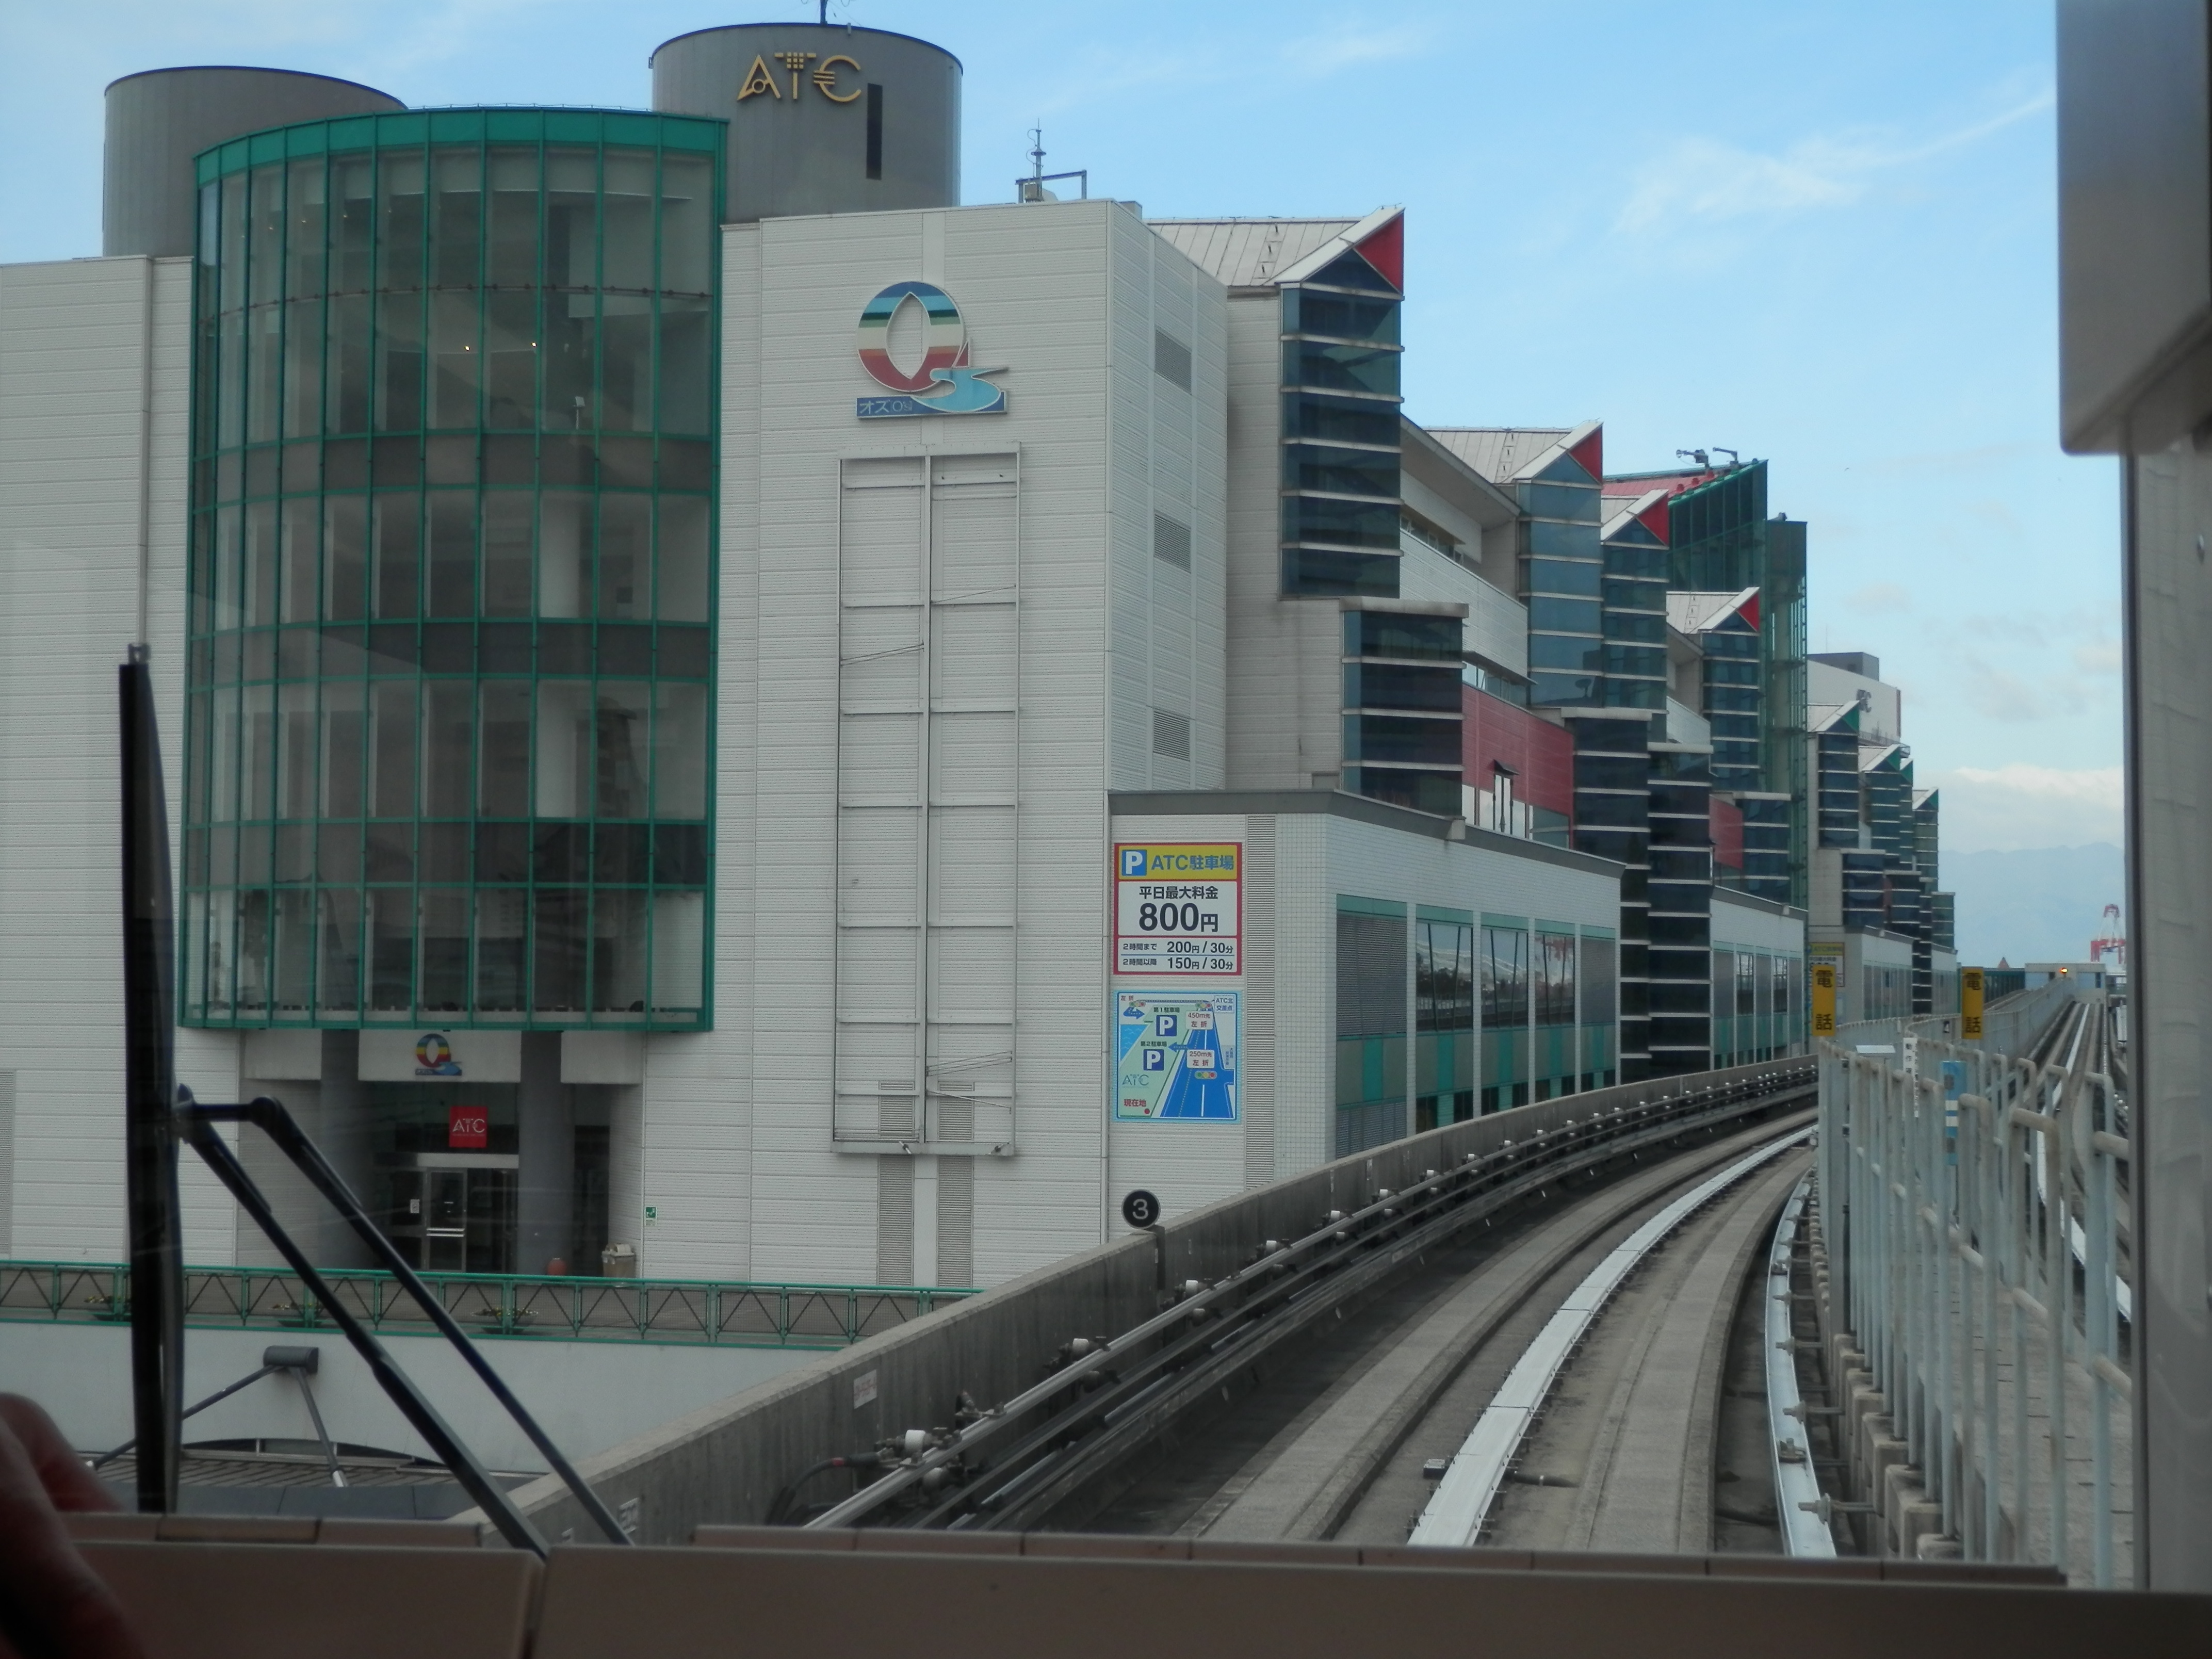
\includegraphics[width=6.5cm]{20121110-atc-os}}\\
	\includegraphics[width=\textwidth]{kof-logo2018-0}\\
%        \resizebox{7cm}{!}{2018年11月9日(金),10日(土)}
}

\date{}

\begin{document}
\maketitle

\thispagestyle{empty}
\pagebreak{}
\section{関西*BSDユーザ会(K*BUG)ってなぁに?}
関西 *BSD ユーザ会 (Kansai *BSD Users Group; K*BUG)とは、
BSD系OSのユーザ同士の情報交換のための{\Large\em \textcolor{red}{場}}で、1999年に設立されました。

年に数度の勉強会やイベントへの参加、そして{\Large\em \textcolor{red}{飲み会}}を行っています。

\subsection{K*BSDの基本理念}
K*BUGの基本理念はのとおりです。

\fbox{\begin{minipage}{\textwidth}
\begin{itemize}
\item 場の提供を目的とする
\item 人のケツは叩くが足は引っ張らない
\item 来るものは拒まず、猿ものは追わず
\item だれでも役員になれる。誰でも役員は止められる
\end{itemize}
\end{minipage}}

少し難しく感じるかもしれないですが、
\textcolor{red}{\bf\Large BSDへの愛と情熱}
があれば、
あなたが
\textcolor{blue}{やりたいと思うことができる場}
がK*BUGなのです。

\section{K*BUG Keywords}
K*BUGでは、以下のようなKeywordに関する発表や展示が行われています。

{\large\bf\textcolor{red}{{BSD}}} (FreeBSD (PC-BSD), NetBSD, OpenBSD, DragonlyBSD, {\footnotesize Mac OS X(?), iOS(??) }, ...)
の更新情報 / 利用方法 / ...,
arch (i386, amd64, arm (Raspberry Pi), macppc, landisk, zaurus, wzero3, hpcmips, netwalker, ipaq, fonera, vax, ...),
kernel hackや新技術 (DTrace, ZFS, シリアルドライバ, ...),
FreeBSD portsってなに? (portsの作り方, redports, ...),
Security (実際のセキュリティ問題に関して, セキュリティを向上するために, ...), 
教育,
いろいろな言語 (Prolog, Lisp, awk, Squeak, Scratch, ...),
OpenCV,
ContaoCMS, 
hardware (UPS, HDD, Server, Bluetooth, GPIO, ...),
ものづくり,
電子工作,
ニコ動技術部 (猫耳サーボ (USB audio servo controler)
, ...),
雑誌付録基板 ,
Physical Computing (Gainer (gainerm-lib), Arduino, ...),
木彫, でーもんくん, でもんむし君 , \\
\hfill{\textcolor{red}{{\bf\large 飲み会}}}, and {\em\textcolor{red}{{ more with }}{\Large\bf\textcolor{red}{{YOU!!}}}}

\newpage
\section{K*BUGの活動}
最近の活動はこんな感じです。
もし、興味のあるテーマがあったら、
\begin{center}
{\huge\bf \textcolor{red}{遊びに来てね!!}}
\end{center}

\subsection{2018年10月13日(土)@大阪 第5回研究会}
\begin{itemize}
\item TVだってコマンドラインでいじりたおしたい:HDMI CEC
\item Cisco CyperOpsはじめました
\item USB0000
\item だべりんぐ
\end{itemize}

\subsection{2018年8月18日(土)@京都 第4回研究会}
\begin{itemize}
\item NetBSD pkginのトラブル
\item ZFS突然死は必然死だったの巻 % \url{http://ds.truefc.org/~kiri/kbug/bof/2018/No.4/}
\item 新ノートを買った ThinkPad X280
\item macOSでpkgsrc
\item OSC 2018 Kyotoのご報告 % \url{https://scrapbox.io/BSD/OSC_2018_Kyotoのご報告(公開版)}
\item 近所のNew comer 新人さんからのQ\&Aタイム
\end{itemize}

\subsection{2018年8月3日(金), 4日(土) @京都 \\\hfill OSC2018 Kyoto}
\begin{itemize}
\item セミナー: 関西*BSDユーザ会研究会番外編
\item ご贈答箱クラスタ: evbarm(arm 32bit) \& aarch64(arm 64bit)
\item PICマイコンで動く!! RetroBSD (2.11BSD) \& LiteBSD (4.4BSD)
\item NetBSD de Blinkt!: ラズパイBSDだってピカピカしたい!!
\item NVIDIA Tegra TK1でCUDA
\item INDIやASCOMによる天文観測
\end{itemize}

\subsection{2018年6月9日(土)@大阪 第3回研究会}
\begin{itemize}
\item ZFS突然死の原因はやはりZFSのバグだった? %\url{http://ds.truefc.org/~kiri/kbug/bof/2018/No.3/}
\item NVIDIA Jetson TX1のご紹介 %\url{https://scrapbox.io/BSD/NVIDIA_Jetson_TX1%E3%81%AE%E3%81%94%E7%B4%B9%E4%BB%8B}
\end{itemize}

\subsection{2018年4月14日(土)@京都 第2回研究会}
\begin{itemize}
\item macOSの小ネタ
\item Dovecotのmmapのエラー
\item Bluetooth心拍計
\item Google Home Mini
\end{itemize}

\subsection{2018年2月10日(土)@大阪 第1回研究会}
\begin{itemize}
\item SG116jに12.0を入れてみた %\url{http://ds.truefc.org/~kiri/kbug/bof/2018/No.1/}
\item Webカメラが動かない
\item NetBSD on C.H.I.P. %\url{http://qml.610t.org/FreeBSD/KBUG_CHIP.html}
\end{itemize}

\subsection{2017年12月9日(土)@大阪\\\hfill 第19回定期総会 + 併設研究会}
\begin{itemize}
\item NanoPi Neo2でNetBSDを動かしたいと思ってたら動いたの %\url{http://qml.610t.org/FreeBSD/KBUG_NanoPiNeo2.html}
\end{itemize}

\subsection{2017年10月14日(土)@京都 第5回研究会}
\begin{itemize}
\item "Hobbes' Internet Timeline"の日本語訳 %\url{https://people.freebsd.org/~kiri/kbug/bof/2017/No.3/}
\item macOS High Sierra雑話
\item daemon(8)話
\item マイコンBSDよもやま
\end{itemize}

\subsection{2017年8月19日(土)@大阪 第4回研究会}

\subsection{2017年6月17日(土)@京都 第3回研究会}

\subsection{2017年4月15日(土)@大阪 第2回研究会}
\begin{itemize}
\item RaSCSIの紹介など
\item sbackup -A Simple Backup script- %\url{https://people.freebsd.org/~kiri/kbug/bof/2017/No.2/}
\item Rasperry PI3 FreeBSD
\item pkgsrc-2017Q1雑談
\end{itemize}

\subsection{2017年2月11日(土)@京都 第1回研究会}

\subsection{2016年12月10日(土)@京都\\\hfill 第18回定期総会 + 併設研究会}
\begin{itemize}
\item Ansibleのお話
\item PostgRESTのお話
\item BHyVeあれこれ %\url{https://people.freebsd.org/~kiri/kbug/bof/2016/No.5/}
\end{itemize}

\section{これからの関連イベント(予定)}
K*BUGでは、2ヶ月に1度程度の頻度で勉強会を行っています。
また、主に関西のイベントで、展示などを行っています。

現在、予定されているイベントは、以下のとおりです。
詳細は、K*BUGのWebページをご確認ください。

\begin{itemize} 
\item 2018年12月8日(土)@京都\\
  \hfill 第20回定期総会 + 併設研究会
\item 2019年も2ヶ月に1度程度の頻度で研究会を行います
\item 2019年1月25日(金),26(土) OSC2019 Osaka
\item 2019年8月2日(金),3日(土) OSC2019 Kyoto (予定)
\end{itemize}

\section{写真集}
\subsection{OSC2018 Kyoto}
  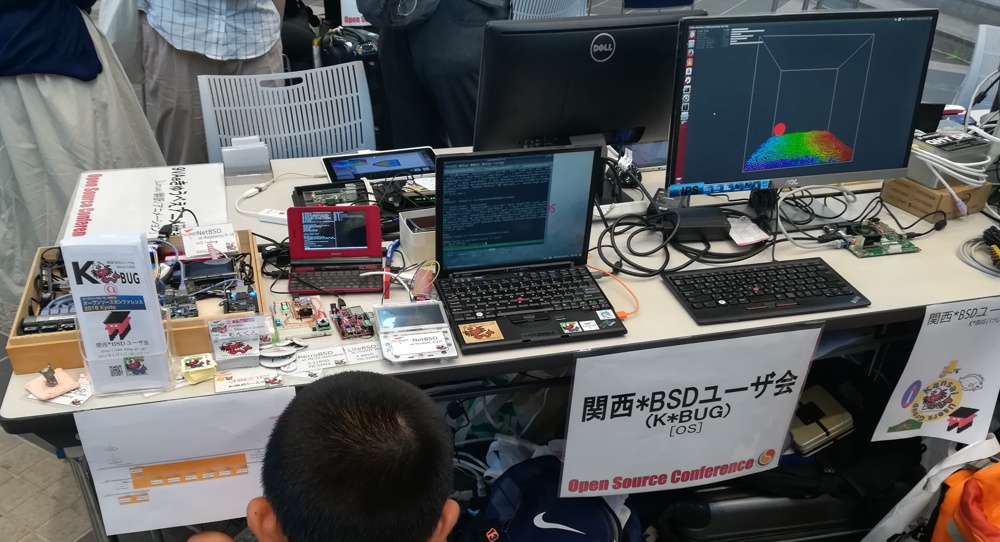
\includegraphics[width=\textwidth]{OSC2018-kyoto-booth}

\subsection{OSC2015 Kansai@Kyoto}
    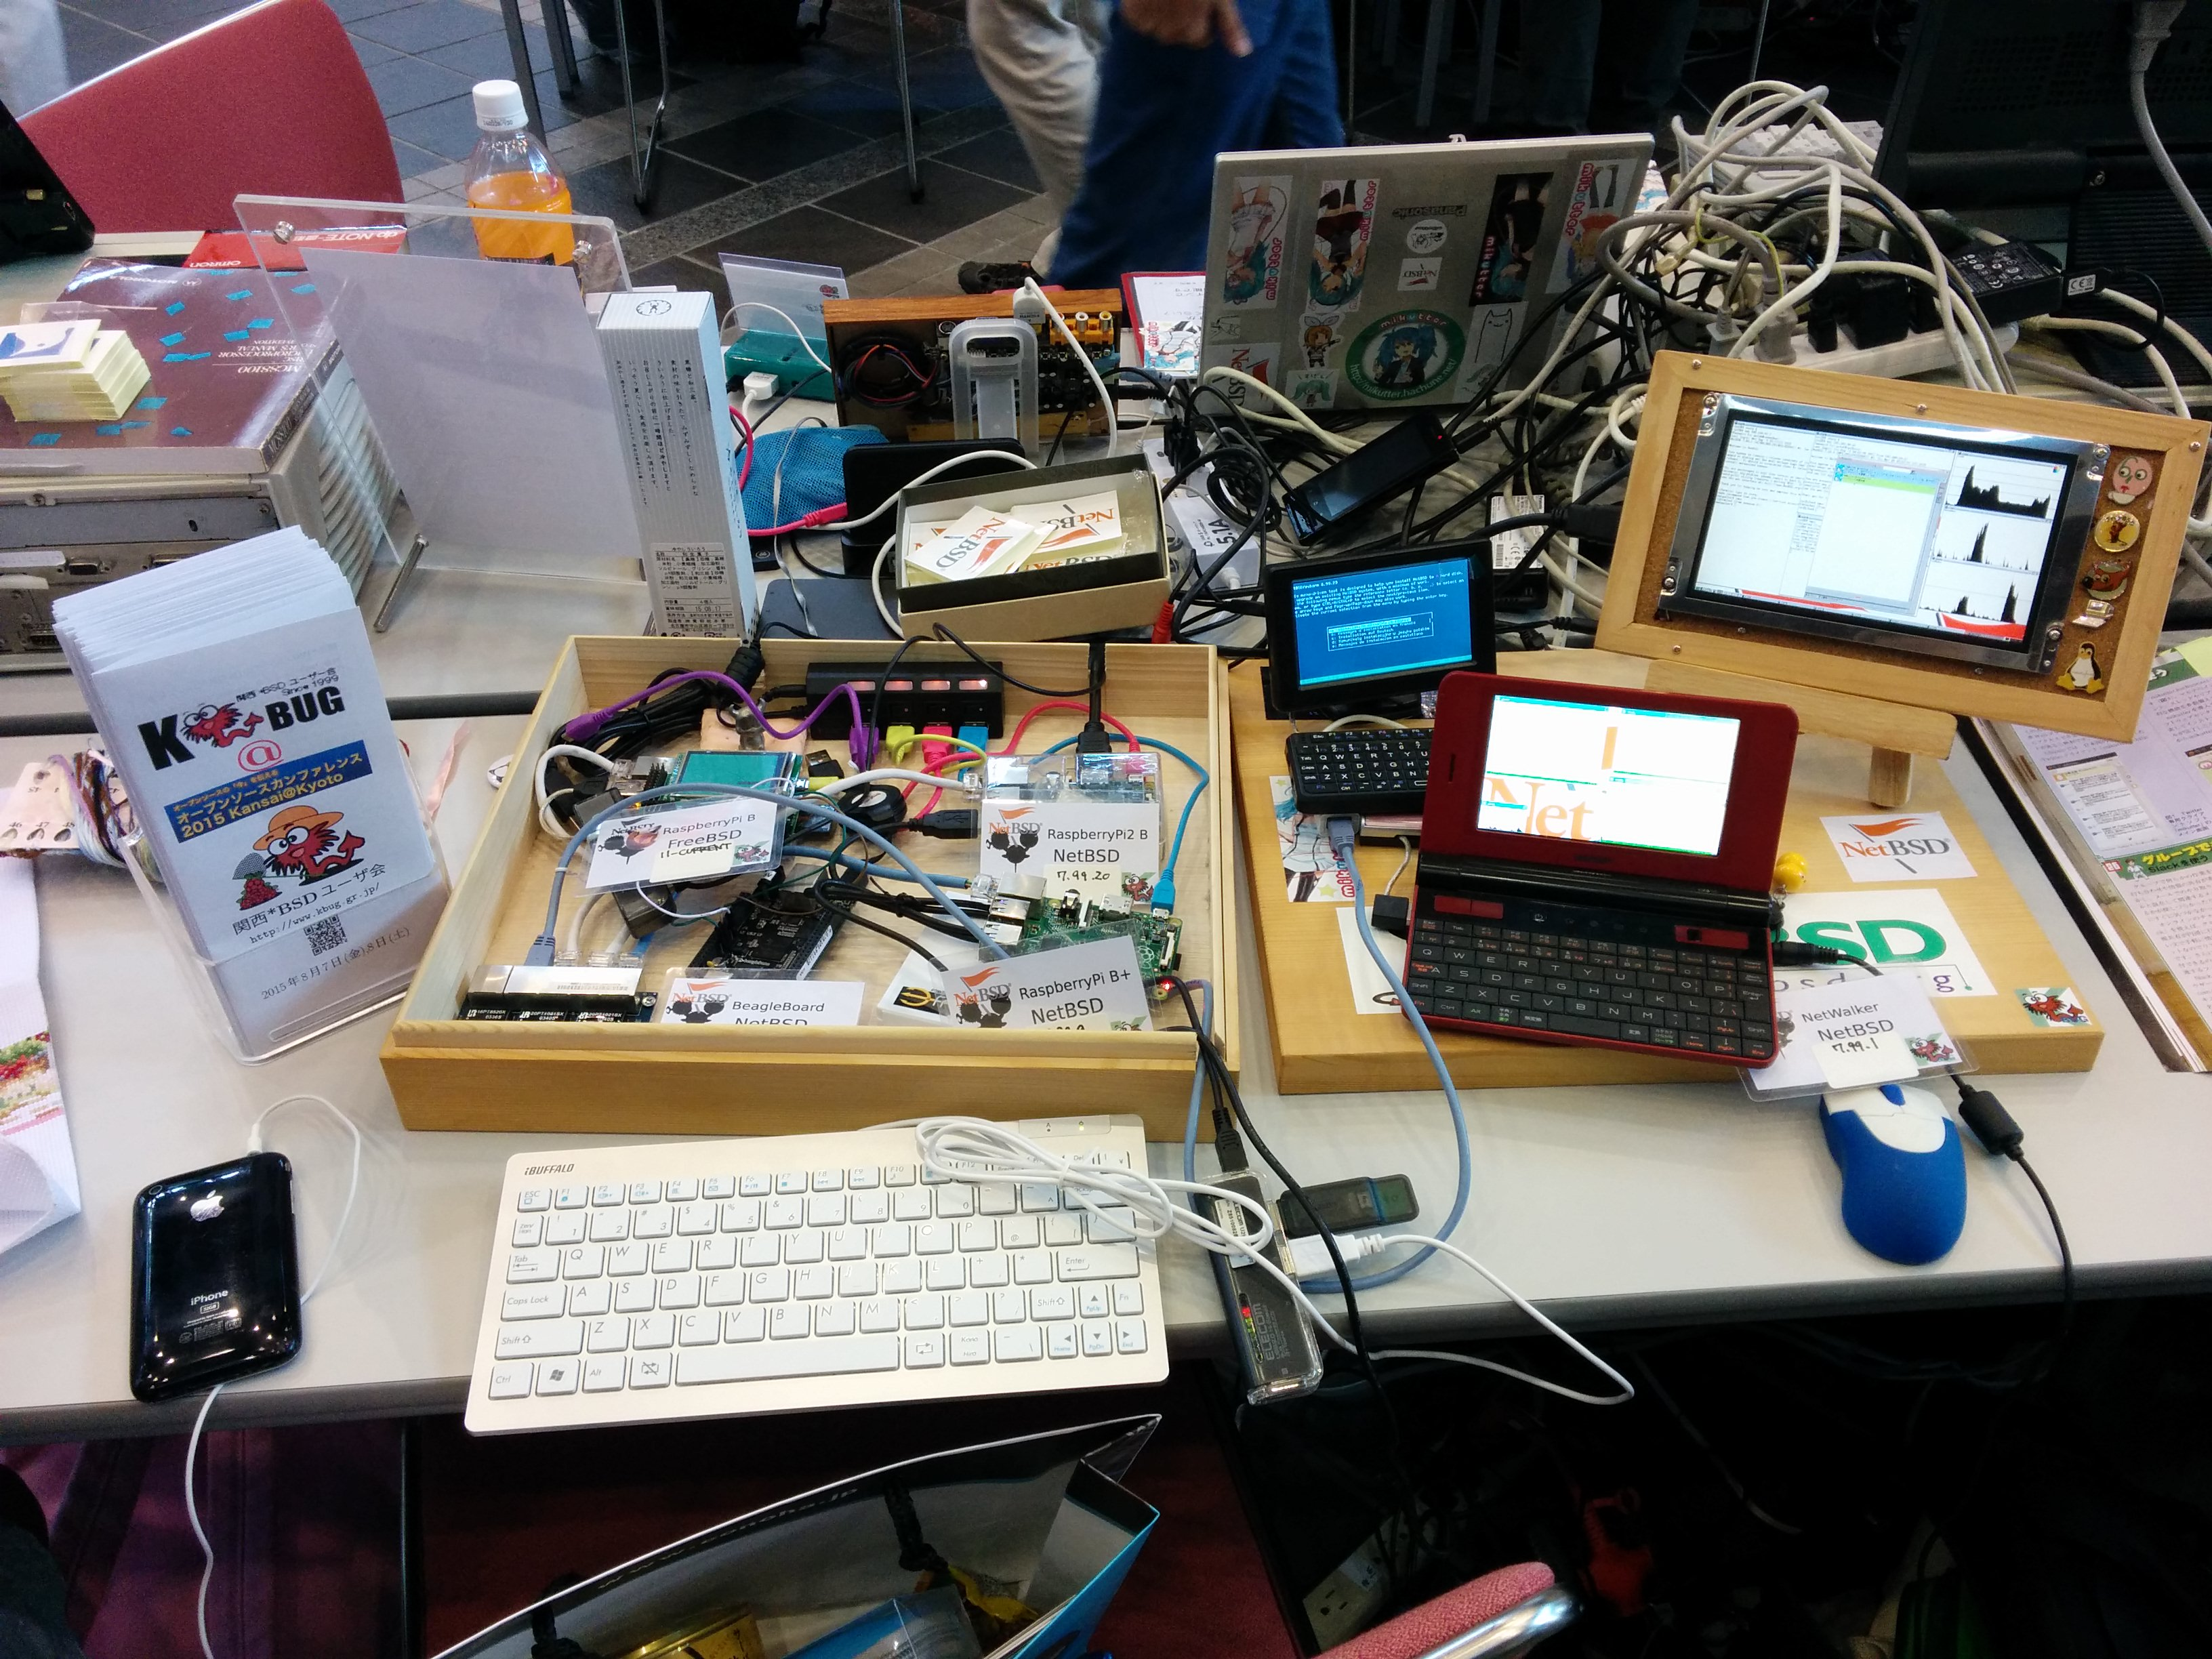
\includegraphics[width=3.5cm]{osc2015-kyoto-booth}
    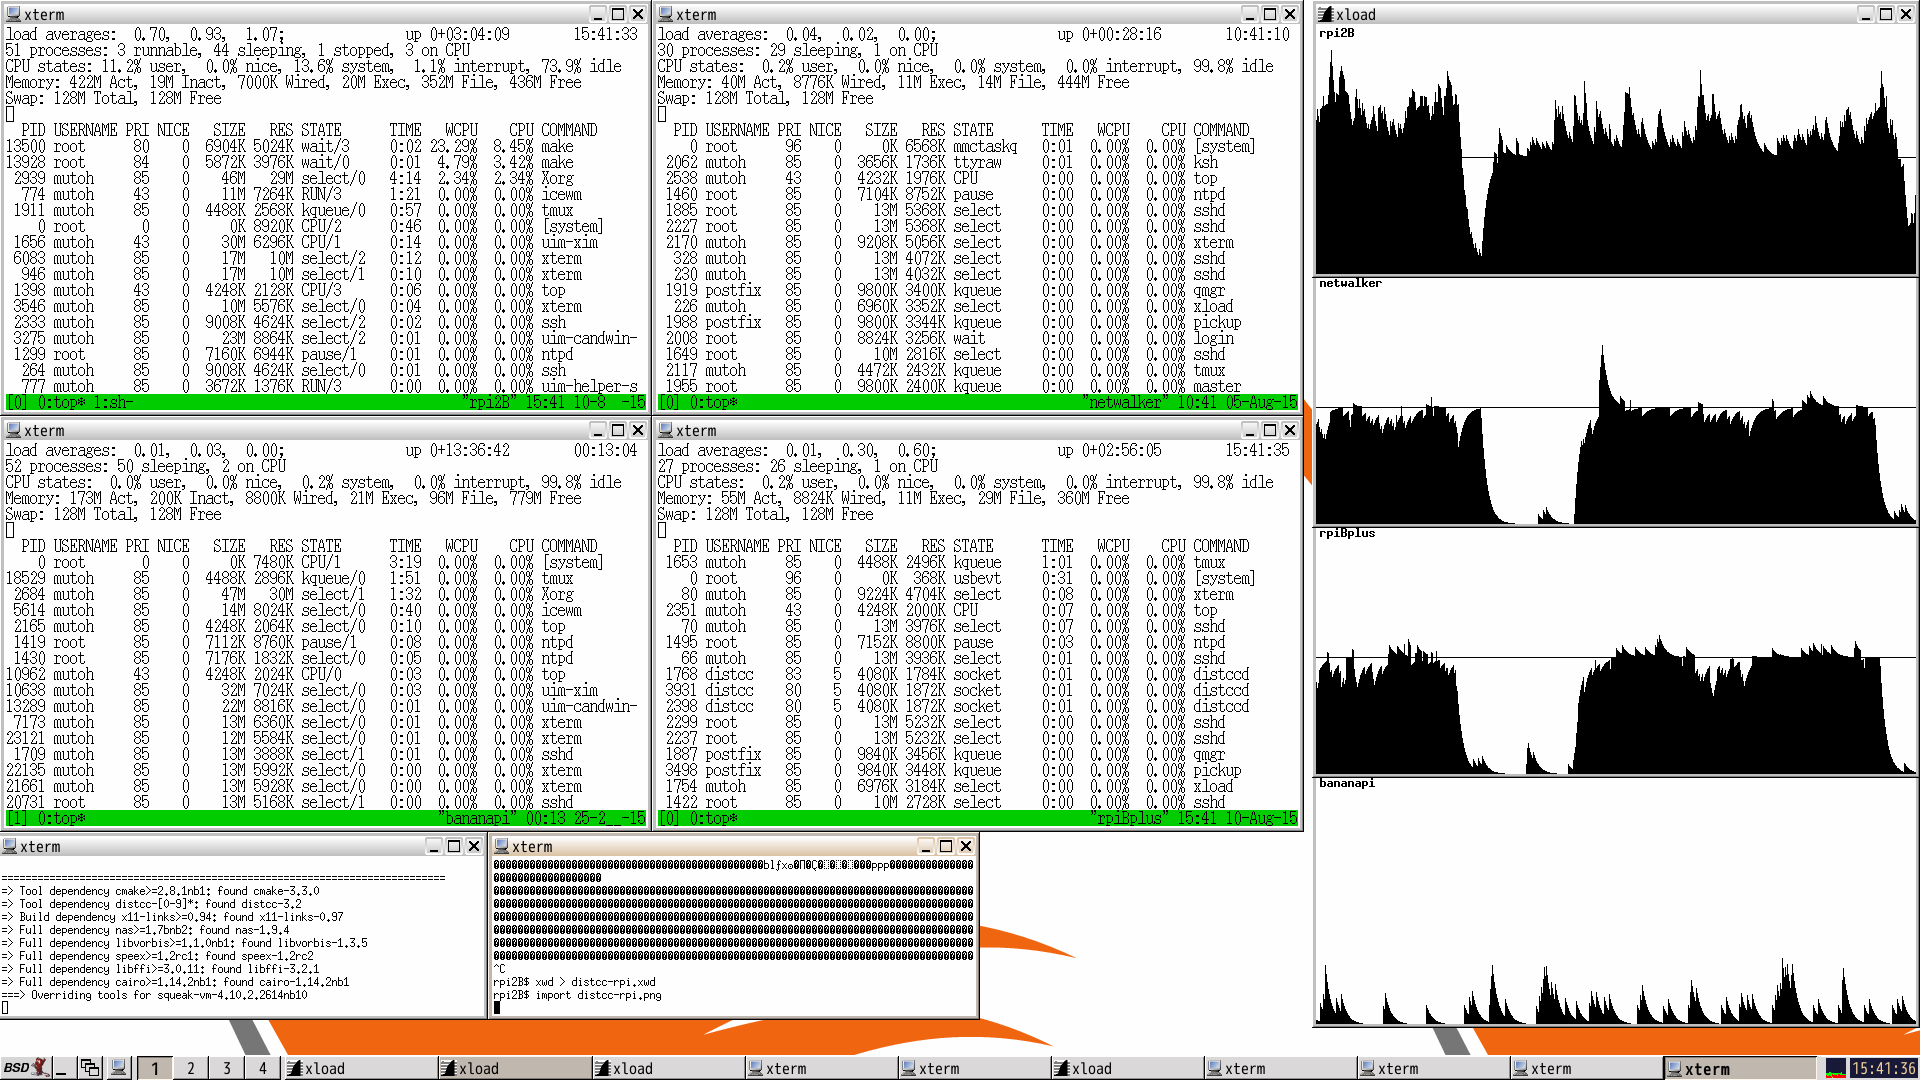
\includegraphics[width=4.5cm]{distcc-rpi}

\newpage
\section{K*BUG @ KOF2018}
%K*BUGは、今回以下のような活動で参加しています。

\subsection{ブース展示関西 *BSDユーザ会}
%以下の様なブース展示を行っています。
\begin{itemize}
\item いろいろなBSDがいっぱい!!
%\item RetroBSDとLiteBSD
%  \footnote{\url{http://qml.610t.org/FreeBSD/OSC2016Kyoto_JNUG.html}}
%  とレトロなBSD
%\item Raspberry Piたちのdistccコンパイルクラスタ
%\item loadavgは愉し
\item このチラシとK*BUGシールを配布してます
\end{itemize}

%\subsection{チラシとシールの配布} % by 日本NetBSDユーザーグループ}

\subsection{セミナー}
\begin{itemize}
\item 日時: 2018年11月9日(金) 13:00-13:50(K*BUG), 15:00-15:50(JNUG)
\item 会場: ショーケース4
\end{itemize}

\subsubsection{関西*BSDユーザ会研究会番外編}
関西*BSDユーザ会は、2ヶ月に1度程度の頻度で、研究会という名前で、BSD UNIXについて語り合う会を行なっています。
今回は番外編としてKOFで研究会を行います。

当日の飛び入りも歓迎しますので、是非面白いBSDネタを発表してください。
\begin{itemize}
\item 講師: 関西 *BSDユーザ会有志など
\item 対象者:BSDに興味がある or 無い人
\end{itemize}

\subsubsection{JNUGセミナー: BSDなひととき}
今年もセミナー枠では「BSD なひととき」をやります。 BSD系UNIXを取り巻く環境と、将来の展望について議論し、 BSDコミュニティ間の情報交換を行なうBOFセッションです。

\begin{itemize}
\item 講師: 蛯原 純(The NetBSD Project,developer )ら
%\item 対象者:コンピュータとかゲーム機とかシャープとかオムロンとか好きな人。
\end{itemize}

%\begin{center}
% 
\includegraphics[width=4cm]{oval-seal-4}
%\end{center}

\vfill
\fbox{\begin{minipage}{\textwidth}

\section{kbug-usersメーリングリスト}
K*BUGでは、K*BUGメンバーの情報交換や、イベントなどの情報伝達用に
kbug-usersメーリングリストを用意しています。

K*BUGメンバーは、基本的にはこのメーリングリストを読んでいることが期待
されます。

購読は、% 右のQRコードを使うか、
このURL
\footnote{\scriptsize \url{http://www.kbug.gr.jp/kbug-mailing-lists.html}}
をご参照ください。
\end{minipage}}
\vfill
\hfill
{\footnotesize\input{date.tex}}
\end{document}
